\begin{center}
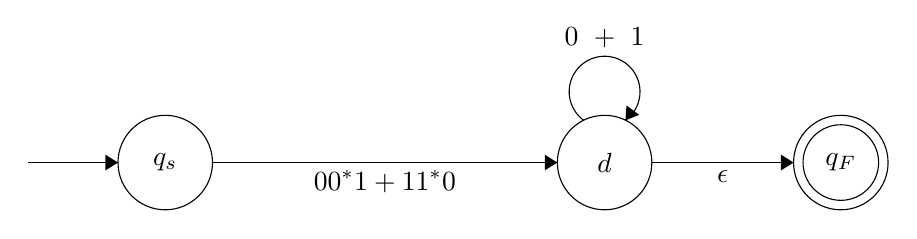
\begin{tikzpicture}[scale=0.2]
\tikzstyle{every node}+=[inner sep=0pt]
\draw [black] (54,-30.4) circle (3);
\draw (54,-30.4) node {$d$};
\draw [black] (69,-30.4) circle (3);
\draw (69,-30.4) node {$q_F$};
\draw [black] (69,-30.4) circle (2.4);
\draw [black] (26.1,-30.4) circle (3);
\draw (26.1,-30.4) node {$q_s$};
\draw [black] (52.677,-27.72) arc (234:-54:2.25);
\draw (54,-23.15) node [above] {$0\mbox{ }+\mbox{ }1$};
\fill [black] (55.32,-27.72) -- (56.2,-27.37) -- (55.39,-26.78);
\draw [black] (57,-30.4) -- (66,-30.4);
\fill [black] (66,-30.4) -- (65.2,-29.9) -- (65.2,-30.9);
\draw (61.5,-30.9) node [below] {$\epsilon$};
\draw [black] (17.4,-30.4) -- (23.1,-30.4);
\fill [black] (23.1,-30.4) -- (22.3,-29.9) -- (22.3,-30.9);
\draw [black] (29.1,-30.4) -- (51,-30.4);
\fill [black] (51,-30.4) -- (50.2,-29.9) -- (50.2,-30.9);
\draw (40.05,-30.9) node [below] {$00^*1+11^*0$};
\end{tikzpicture}
\end{center}